\documentclass{beamer}
\usepackage{pgffor,pgfmath}
\usepackage{lipsum}
\usepackage{multicol}
\usetheme{ucla}
\usepackage{graphicx}
\usepackage{listings}
\usepackage{verbatim}
\usepackage{tikz}
\linespread{1.5}
\usepackage{comment}

\usepackage{amsmath, amsthm, amssymb, latexsym}

%\newtheorem{definition}{Definition}

\title{Lecture 8}
\author{Charles Rambo}
\institute{UCLA Anderson School of Management}
\date{2023}
\location{Los Angeles, California}

% Turn on slide numbers:
\showSlideNumber{}

\AtBeginSection[]
{
    \begin{frame}
        \frametitle{Table of Contents}
        \tableofcontents[currentsection]
    \end{frame}
}


\begin{document}

\insertTitleSlide

\section{Probability}

\subsection{Continuous Random Variable}

\begin{frame}
\frametitle{Continuous Random Variable}
\begin{Definition}
We say that a random variable $X$ is {\bf continuous} if there exists a non-negative function $f$ defined for all real numbers and having the property that for any set $B$ of real numbers we have
$$
P(X\in B) = \int_B f(x)\ dx.
$$
The function $f$ is called the {\bf probability density function} or {\bf pdf} of the random variable $X$.
\end{Definition}

\end{frame}

\begin{frame}
\frametitle{Diagram}
\begin{center}
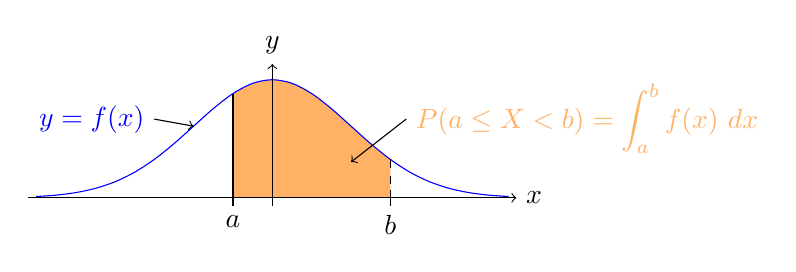
\begin{tikzpicture}[declare function = {normal(\x) = 1.5 * exp(-0.5 * \x * \x);}, ]

% Shade orange area underneath curve.
\fill [fill=orange!60] (-0.5, 0) -- plot[domain= -0.5:1.5] (\x, {normal(\x)}) -- (1.5 ,0) -- cycle;

% Draw and label normal distribution function
\draw[color=blue, domain=-3:3, smooth] plot (\x, {normal(\x)});

% Draw line
\draw (-0.5, {normal(-0.5)}) -- (-0.5, 0);
\draw (-0.5, 0.1) -- (-0.5, -0.1) node[below] {$a$}; 

% Add dashed line dropping down from normal.
\draw[dashed] (1.5, {normal(1.5)})  -- (1.5, 0);
\draw (1.5, 0.1) -- (1.5, -0.1) node[below] {$b$};

\draw[->] (-3.1, 0) -- (3.1, 0) node[right] {$x$};
\draw[->] (0, -0.1) -- (0, 1.7) node[above] {$y$};

\draw [<-] (1, {0.5 * normal(1)}) -- (1.7, 1) node[right] {$\textcolor{orange!60}{ P(a\leq X < b) = \displaystyle\int_a^b f(x)\ dx}$};
\draw[<-] (-1, {normal(-1)}) -- (-1.5, 1) node[left] {$\textcolor{blue}{y = f(x)}$};

\end{tikzpicture}
\end{center}
\end{frame}

\begin{frame}
\frametitle{Cumulative Distribution Function}
\begin{Definition}
The {\bf cumulative distribution function} or {\bf cdf} of a random variable $X$ is defined to be
$$
F(x) = P(X \leq x) = \int_{-\infty}^x f(t)\ dt,
$$
where $f$ is the pdf of $X$.
\end{Definition} 

\end{frame}

\begin{frame}
\frametitle{Properties of the CDF}
\small
The cumulative distribution function $F$ of a continuous random variable $X$ satisfies the following properties.
\begin{enumerate}
\item[(a)] $0 \leq F(x) \leq 1$
\item[(b)] If $x_1 < x_2$, then $F(x_1) < F(x_2)$
\item[(c)] $\displaystyle\lim_{x\to-\infty} F(x) = 0$
\item[(d)] $\displaystyle\lim_{x\to\infty} F(x) = 1$
\item[(e)] $P(a < X \leq b) = F(b) - F(a)$
\item[(f)] $F$ is continuous 
\item[(g)] $F\;'(x) = f(x)$ wherever the derivative exists.
\end{enumerate}
\end{frame}

\begin{frame}[t]
\frametitle{PDF and CDF Example}
\begin{Example}
Suppose a random variable $X$'s pdf is proportional to $x^2$ on the interval $[-1, 2]$ and 0 elsewhere. Find the pdf and cdf of $X$.
\end{Example}

\end{frame}

\begin{frame}
\frametitle{The Continuous Uniform Distribution} 
\small 
\begin{Definition}
The {\bf continuous uniform distributions} describes an experiment where there is an arbitrary outcome that lies between certain bounds. The bounds are defined by the parameters $a$ and $b$, which are the minimum and maximum values. The interval can either be closed or open. The distribution is often abbreviated $\mathcal{U}(a, b)$. 
\end{Definition}
The pdf and cdf of the continuous uniform distribution are
$$
f(x) = \begin{cases} \displaystyle\frac{1}{b - a},	&	a\leq x\leq b\\ 0, & \text{otherwise}\end{cases}\qquad\text{and}\qquad F(x) = \begin{cases} 0,	&	x < a\\ \displaystyle\frac{x}{b - a}, & 	a\leq x\leq b\\	1,	&	x > b.\end{cases}
$$
\end{frame}

\begin{frame}[t]
\frametitle{Continuous Uniform Distribution Example}
\begin{Example}
Suppose that $X\sim{\mathcal{U}(0, b)}$, where $b > 1$. Find $P(X^2 < X)$.
\end{Example}

\end{frame}

\begin{frame}
\frametitle{Normal Distribution}
\begin{Definition}
The {\bf normal} or {\bf Gau{\ss}ian distribution} has probability density function 
$$
\displaystyle f(x) = \frac{1}{\sigma \sqrt{2\pi}} e^{-\frac{1}{2}\left(\frac{x - \mu}{\sigma}\right)^2}.
$$
The parameters of the distribution are $\mu$ and $\sigma^2$. To denote that $X$ follows a normal distribution, we write $X\sim{\mathcal{N}(\mu, \sigma^2)}$.
\end{Definition} 
\end{frame}

\begin{frame}[fragile]
\frametitle{Normal Python Example}
\small
\begin{Example}
Use Python to illustrate how $\mu$ and $\sigma$ affect the graph of the pdf.
\end{Example}

{\bf Solution.}
{
\linespread{0.8}
\tiny
\begin{verbatim*}
import numpy as np, matplotlib.pyplot as plt
from scipy.stats import norm

# Use latex
plt.rcParams['text.usetex'] = True

# Use Seaborn style
plt.style.use('seaborn')

# Mu- and sigma-values
mu_vals, sigma_vals = [-2, 0, 1], [0.5, 1, 1.5]

# Set up subplots
fig, ax = plt.subplots(1, 2, sharey = True, figsize = (10, 6))

# Get x-values
x_vals = np.linspace(-4.5, 3.5, 100)
\end{verbatim*}
}

\end{frame}

\begin{frame}[fragile]
\frametitle{Normal Python Example Continued}
{
\linespread{0.8}
\tiny
\begin{verbatim*}
# Loop over mu-values
for mu in mu_vals:

    y_vals = [norm.pdf(x, loc = mu, scale = 1) for x in x_vals]
    
    ax[0].plot(x_vals, y_vals, label = r'$\mu =$ ' + str(mu))

# Create legend for first subplot
ax[0].legend()

# Loop over sigma-values
for sigma in sigma_vals:
    
    y_vals = [norm.pdf(x, loc = 0, scale = sigma) for x in x_vals]
    
    ax[1].plot(x_vals, y_vals, label = r'$\sigma =$ ' + str(sigma))

# Create legend for second subplot
ax[1].legend()

# Save the figure
plt.savefig(r'[location on machine]')

# Show plot
plt.show()
\end{verbatim*}
}
\end{frame}

\begin{frame}[fragile]
\frametitle{Normal Python Example Result}

\begin{center}
\includegraphics[scale = 0.50]{ex9.png}
\end{center}

\end{frame}

\begin{frame}
\frametitle{Standard Normal Distribution}
\begin{Definition}
The {\bf standard normal distribution} is $\mathcal{N}(0, 1^2)$, i.e. it is a normal distribution with $\mu = 0$ and $\sigma^2 = 1$. The pdf and cdf are sometimes denoted $\phi$ and $\Phi$, respectively. 
\end{Definition}
You can translate a normal random variable into a standard normal variable by calculating its $Z$-score:
$$
X\sim{\mathcal{N}(\mu, \sigma^2)}\qquad\text{implied}\qquad Z = \frac{X - \mu}{\sigma}\sim{\mathcal{N}(0, 1^2)}.
$$
\end{frame}


\begin{frame}
\frametitle{Empirical Rule}
\small
\begin{center}
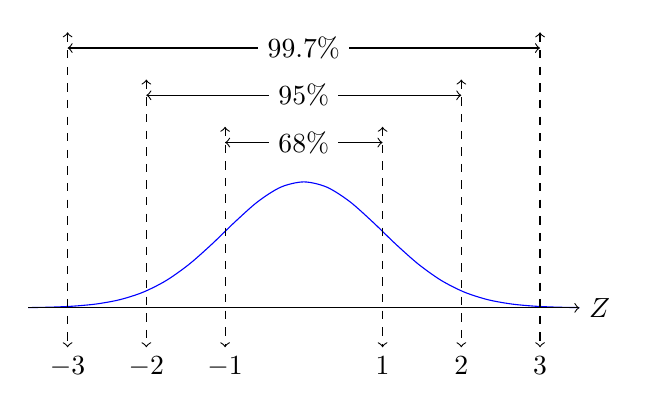
\begin{tikzpicture}[declare function = {normal(\x) = 1.6 * exp(-0.5 * \x * \x);}, ]
% Draw and label normal distribution function
\draw[color=blue, domain=-3.5:3.5, smooth] plot (\x, {normal(\x)});


\draw[->] (-3.5, 0) -- (3.5, 0) node[right] {$Z$};


\draw[dashed, <->] (-1, 2.3) -- (-1, -0.5) node[below] {$-1$};
\draw[dashed, <->] (1, 2.3) -- (1, -0.5) node[below] {$1$};

\draw[<->] (-1, 2.1) -- (1, 2.1);
\node[fill = white] at (0, 2.1) {$68\%$};


\draw[dashed, <->] (-2, 2.9) -- (-2, -0.5) node[below] {$-2$};
\draw[dashed, <->] (2, 2.9) -- (2, -0.5) node[below] {$2$};

\draw[<->] (-2, 2.7) -- (2, 2.7);
\node[fill = white] at (0, 2.7) {$95\%$};


\draw[dashed, <->] (-3, 3.5) -- (-3, -0.5) node[below] {$-3$};
\draw[dashed, <->] (3, 3.5) -- (3, -0.5) node[below] {$3$};

\draw[<->] (-3, 3.3) -- (3, 3.3);
\node[fill = white] at (0, 3.3) {$99.7\%$};

\end{tikzpicture}
\end{center}
If $Z\sim{\mathcal{N}(0, 1^2)}$, then
$$
P(|Z| < 1) \approx 68\%,\qquad P(|Z| < 2) \approx 95\%,\qquad\text{and}\qquad P(|Z| < 3) = 99.7\%.
$$
\end{frame}

\begin{frame}[t]
\frametitle{Normal Distribution Example}
\begin{Example}
Suppose that the daily returns for a stock index $R\sim{\mathcal{N}{(0, 0.01^2)}}$. What is the probability of this index dropping more than 3\%?
\end{Example}

\end{frame}

\begin{frame}
\frametitle{Exponential Distribution}
\small
\begin{Definition}
The {\bf exponential distribution} describes an experiment where events occur continuously and independently at a constant average rate $\lambda$. Exponential random variables are often used to model arrival times, waiting
times, and equipment failure times.
\end{Definition}
To denote that the random variable $X$ follows and exponential distribution, we write $X\sim{\mathcal{E}(\lambda)}$. The pdf and cdf of an exponential distribution are
$$
f(x) = \begin{cases} 0, & x < 0\\ \lambda e^{-\lambda x},& x\geq 0\end{cases} \qquad\text{and}\qquad F(x) = \begin{cases} 0,	&	x < 0\\ 1 - e^{-\lambda x},&	x\geq 0.\end{cases}
$$

\end{frame}

\begin{frame}[t]
\frametitle{Exponential Distribution Example}
\begin{Example}
Suppose that the time until default, measured in years, of a firm $T$ follows an exponential distribution with $\lambda = 0.10$. What is the probability that $2 < T < 5$?
\end{Example}

\end{frame}

\subsection{Expected Value}

\begin{frame}
\frametitle{Expected Value}
\begin{Definition}
The {\bf expected value} of a discrete random variable $X$ is
$$
E[X] = \mu_X = \sum_x xP(x),
$$
where we sum over the range of $X$. If $X$ is a continuous random variable, then the expected value is
$$
E[X] = \mu_X = \int_{-\infty}^\infty x f(x)\ dx.
$$
\end{Definition}
\end{frame}

\begin{frame}
\frametitle{Property of Expected Value}
For random variables $X$ and $Y$, and scalars $\alpha$ and $\beta$, we have
$$
E[\alpha X + \beta Y] = \alpha E[X] + \beta E[Y].
$$
\end{frame}

\begin{frame}[t]
\frametitle{Expected Value Example}
\begin{Example}
Suppose that the pmf of $N$ is
$$
p(n) = \begin{cases} \left(\frac{1}{2}\right)^n,	&	n = 1, 2 \ldots\\ 0,	&\text{otherwise.}\end{cases}
$$
Calculate $E[N]$.
\end{Example}
\end{frame}


\begin{frame}
\frametitle{Variance and Standard Deviation}
\begin{Definition}
The {\bf variance} of a discrete random variable $X$ is
$$
\text{Var}(X) = \sigma_X^2 = \sum_x \left(x - \mu_X \right)^2 p(x).
$$
If $X$ is a continuous random variable
$$
\text{Var}(X) = \sigma_X^2 = \int_{-\infty}^\infty \left(x - \mu_X\right)^2 f(x)\ dx.
$$
The {\bf standard deviation} of $X$ is the square root of its variance and is denoted by $\sigma_X$.
\end{Definition}
\end{frame}

\begin{frame}[t]
\frametitle{Variance Example}
\begin{Example}
Prove the identity 
$$
\text{Var}(X) = E[X^2] - \left(E[X]\right)^2.
$$
\end{Example}
\end{frame}

\begin{frame}
\frametitle{Property of Variance}
For random variable $X$ and scalars $\alpha$ and $\beta$
$$
\text{Var}\left(\alpha X + \beta\right) = \alpha^2 \text{Var}(X).
$$
\end{frame}

\begin{frame}
\frametitle{Expected Value and Variance Formulas}

\begin{tabular}{ | c |	c	c | }
\hline
\text{Distribution}			&	\text{Expected Value}					&	\text{Variance}\\\hline
						&										&				\\
Discrete Uniform			&	$\displaystyle\frac{1}{n} \sum_{k = 1}^n x_k$	&	$\displaystyle\frac{1}{n} \sum_{k = 1}^n x_k^2 - \left(\frac{1}{n} \sum_{k = 1}^n x_k\right)^2$\\
$\mathcal{B}(n, p)$			&	$np$									&	$np(1 - p)$\\
$\mathcal{P}(\lambda)$		&	$\lambda$								&	$\lambda$\\
$\mathcal{U}(a, b)$			&	$\displaystyle\frac{b + a}{2}$				&	$\displaystyle\frac{(b - a)^2}{12}$		\\
$\mathcal{N}(\mu, \sigma^2)$	&	$\mu$								&	$\sigma^2$						\\
$\mathcal{E}(\lambda)$		&	$\displaystyle\frac{1}{\lambda}$				&	$\displaystyle\frac{1}{\lambda^2}$		\\
						&										&									\\\hline
\end{tabular}

\end{frame}

\subsection{Moments}

\begin{frame}
\frametitle{$\boldsymbol k$-th Moment}
\begin{Definition}
If $X$ is a random variable, then its $\boldsymbol k$-th moment is $E[X^k]$.
\end{Definition}

\begin{Definition}
The {\bf moment generating function} of a random variable $X$ is
$$
\psi(t) = E[e^{tX}].
$$
\end{Definition}
We call $\psi$ the moment generating function of $X$ because
$$
E[X^k] = \psi^{(k)}(0).
$$
\end{frame}

\begin{frame}[t]
\frametitle{Moment Generating Function Example}
\begin{Example}
Find the moment generating function of $X$, the discrete uniform distribution with support $\{1, 2, 3\}$.
\end{Example}

\end{frame}

\subsection{Function of a Random Variable}

\begin{frame}[fragile]
\frametitle{Function of a RV Python Example}
\small
\begin{Example}
Suppose $Z\sim{\mathcal{N}(0, 1)}$. Consider $X = Z^2$. Use Python to approximate the graph of the pdf of $X$ using a histogram. 
\end{Example}

{\bf Solution.}
{
\linespread{0.8}
\tiny
\begin{verbatim*}
# Import modules
import numpy as np, matplotlib.pyplot as plt
from scipy.stats import norm

# Use latex
plt.rcParams['text.usetex'] = True

# Use Seaborn style
plt.style.use('seaborn')

# Generate Z
Z = norm.rvs(size = 10000)

# Calculate X
X = Z**2

# Generate histogram; make sure density is True
plt.hist(X, bins = 100, density = True)

# Get title 
plt.title(r'Histogram of $X = Z^2$')

# Save the figure
plt.savefig(r'[location on machine]')

plt.show()
\end{verbatim*}
}


\end{frame}

\begin{frame}
\frametitle{Function of a Random Variable Python Result}
\small 
This is a known distribution $\chi^2(1)$. See \href{https://en.wikipedia.org/wiki/Chi-squared_distribution}{Wikipedia} for more details. 
\begin{center}
\includegraphics[scale = 0.40]{ex10.png}
\end{center}

\end{frame}

\begin{frame}
\frametitle{Function of a Random Variable}
This result can be obtained analytically by considering the cdf and differentiating. 
\end{frame}

\begin{frame}[t]
\frametitle{Function of a Random Variable Example}
\begin{Example}
Suppose $Z\sim{\mathcal{N}(0, 1)}$. Consider $X = Z^2$. Calculate the pdf of $X$.
\end{Example}

\end{frame}

\begin{frame}
\frametitle{Functions of a Random Variable Theorem}

\begin{Theorem}
Let $X$ be a random variable with pdf $f$. Suppose $P(a < x < b) = 1$. Let $Y = r(X)$ and suppose $r$ is differentiable and one-to-one for $a < x < b$. Let the image of $(a, b)$ under $r$ be $(\alpha, \beta)$. If $s$ is the inverse of $r$, then the pdf of $Y$ is
$$
g(y) = \begin{cases} f\left(s(y)\right)\left|\frac{ds}{dy}\right|,	&	\alpha < y <\beta\\ 0,	&	\text{otherwise.}\end{cases}
$$
\end{Theorem}

\end{frame}

\begin{frame}[t]
\frametitle{Functions of a Random Variable Example}
\begin{Example}
Suppose $X\sim{\mathcal{U}(0, 1)}$ and let $Y = \frac{1}{27}X^3$. Find the pdf of $Y$.
\end{Example}

\end{frame}


\subsection{Joint Distribution} 

\begin{frame}

\frametitle{Joint Distribution}
\begin{Definition}
Two random variables $X$ and $Y$ are said to be {\bf jointly continuous} if there exists a function $f_{XY}(x, y) \geq 0$ with the property that for every subset $C$ of $\mathbb{R}^2$, we have
$$
P\Big((X, Y)\in C\Big) = \iint_C f_{XY}(x, y)\ dA.
$$
The function $f_{XY}(x, y)$ is called the {\bf joint probability density function} of $X$ and $Y$, and the {\bf joint cumulative distribution function} is
$$
F(x, y) = \int_{-\infty}^y\int_{-\infty}^x f(s, t)\ dsdt.
$$
\end{Definition}

\end{frame}

\begin{frame}[t]
\frametitle{Joint Distribution Example}
\begin{Example}
\small
Suppose
$$
f_{XY}(x, y) = \begin{cases} \frac{1}{4},	&	-1\leq x, y \leq 1\\ 0,&	\text{otherwise.}\end{cases}
$$
Then $P(2X - Y > 0) = $
\end{Example}

\end{frame}

\begin{frame}
\frametitle{Marginal PDF}
The marginal pdfs of $X$ and $Y$ given joint pdf $f_{XY}$ are
$$
f_X(x) = \int_{-\infty}^\infty f(x,y)\ dy\qquad\text{and}\qquad f_Y(y) = \int_{-\infty}^\infty f(x, y)\ dx.
$$
\end{frame}

\begin{frame}
\frametitle{Independent Events}
If the random variables $X$ and $Y$ are independent, then
$$
f_{XY}(x, y) = f_X(x) f_Y(y).
$$
\end{frame}

\begin{frame}[t]
\frametitle{Independent Events Example}
\small
\begin{Example}
The joint pdf of $X$ and $Y$ is given by
$$
f_{XY}(x, y) = \begin{cases} 3(x + y),&	0\leq x +y \leq 1, 0 \leq x, y\\ 0, & \text{otherwise.}\end{cases}	
$$
Are $X$ and $Y$ independent? 
\end{Example}

\end{frame}

\begin{frame}
\frametitle{Change of Variables}
\tiny
\begin{Theorem}
Let $X$ and $Y$ be continuous random variables with joint density $f_{XY}$. Assume that there is a subset $S$ of $\mathbb{R}^2$ such that
$P\Big((X, Y)\in S\Big) = 1$. Let 
$$
U = r_1(X, Y)\qquad\text{and}\qquad V = r_2(X, Y),
$$ 
where $r_1$ and $r_2$ are one-to-one differentiable transformations from $S$ onto some subset $T$ of $\mathbb{R}^2$. If 
$$
X = s_1(U, V)\qquad\text{and}\qquad Y = s_2(U, V)
$$ 
describe the inverse transformation, where $s_1$ and $s_2$ are also one-to-one and differentiable. Then the joint pdf of $U$ and $V$ is
$$
g_{UV}(u, v) = \begin{cases} f_{XY}\Big(s_1(u, v), s_2(u, v)\Big)\left|\text{det}(J)\right|,	&	(u, v)\in T\\ 0,&	\text{otherwise.}\end{cases}
$$
where 
$$
J = \left(\begin{array}{c c} \dfrac{\partial s_1}{\partial u}	&	\dfrac{\partial s_1}{\partial v}\\ \dfrac{\partial s_2}{\partial u}	&	\dfrac{\partial s_2}{\partial v}\end{array}\right)
$$
is the Jacobian.
\end{Theorem}

\end{frame}

\begin{frame}[t]
\frametitle{Change of Variables Example}
\begin{Example}
Suppose $f_{XY}(x, y) = \frac{1}{2\pi} e^{-\frac{x^2 + y^2}{2}}$. Find the joint pdf of $r$ and $\theta$, where $x = r\cos\theta$ and $y=r\sin\theta$.
\end{Example}
\end{frame}

\subsection{Covariance}
\begin{frame}
\frametitle{Covariance}
\begin{Definition}
Let $X$ and $Y$ be random variables having finite means. Suppose $E[X] = \mu_X$ and $E[Y] = \mu_Y$. The {\bf covariance of $\boldsymbol X$ and $\boldsymbol Y$} is
$$
\text{Cov}(X, y) = E\Big[(X - \mu_X)(Y - \mu_Y)\Big].
$$
\end{Definition}
A useful identity is
$$
\text{Cov}(X, Y) = E[XY] - E[X]E[Y].
$$
\end{frame}

\begin{frame}[t]
\frametitle{Covariance Example}
\tiny
\begin{Example}
Consider $X$ and $Y$ with joint pdf
$$
f_{XY}(x, y) = \begin{cases} 2, &	0\leq x \leq y\leq 1\\ 0,	&	\text{otherwise.}\end{cases}
$$
Calculate the covariance of $X$ and $Y$. Hint: $E[X] = E[Y] =  \frac{2}{3}.$
\end{Example}

\end{frame}

\begin{frame}
\frametitle{Properties of Covariance}
Suppose $X_i$ and $Y_j$ are random variables for all $i$ and $j$, and $\alpha$ is a real number
\begin{enumerate}
\item[(a)] $\text{Cov}(X_1, X_2) = \text{Cov}(X_2, X_1)$
\item[(b)] $\text{Cov}(X_1, X_1) = \text{Var}(X_1)$
\item[(c)] $\text{Cov}(\alpha X_1, X_2) = \alpha \text{Cov}(X_1, X_2)$
\item[(d)] $\displaystyle \text{Cov}\left(\sum_{i = 1}^m X_i, \sum_{j = 1}^n Y_j\right) = \sum_{i = 1}^m\sum_{j = 1}^n \text{Cov}(X_i, Y_j)$
\end{enumerate}

\end{frame}

\begin{frame}
\frametitle{Correlation}
\begin{Definition} 
Let $X$ and $Y$ be random variables with finite variances $\sigma_X^2$ and $\sigma_Y^2$, respectively. Then the {\bf correlation of $\boldsymbol X$ and $\boldsymbol Y$} is
$$
\rho(X, Y) = \frac{\text{Cov}(X, Y)}{\sigma_X\sigma_Y}.
$$
\end{Definition}

\end{frame}

\begin{frame}[t]
\frametitle{Correlation Example}
\begin{Example}
Suppose $X\sim{\mathcal{U}(-1, 1)}$. Calculate the correlation between $X$ and $X^2$.
\end{Example}

\end{frame}

\begin{frame}
\frametitle{Variance of Sum}

\begin{Theorem}
If $X$ and $Y$ are random variables and $\alpha$ and $\beta$ are constants, then
$$
\text{Var}(\alpha X + \beta Y) = \alpha^2 \text{Var}(X) + \beta^2\text{Var}(Y) + 2\alpha\beta \text{Cov}(X, Y).
$$
\end{Theorem}
\end{frame}

\begin{frame}[t]
\frametitle{Variance of Sum Example}
\begin{Example}
Suppose $X\sim{\mathcal{U}(-1, 1)}$. Calculate the variance of $X - 2 X^2$.
\end{Example}

\end{frame}





\end{document}